\documentclass[10pt]{article}
\usepackage[margin=2.2cm]{geometry}
\usepackage{amsmath,amssymb,amsthm,bm}
\usepackage{booktabs,array,tabularx,graphicx,float}
\graphicspath{{../figures/results/}}
\usepackage[hidelinks]{hyperref}
\usepackage{microtype,placeins}
\pdfsuppresswarningpagegroup=1
\renewcommand{\thesection}{S\arabic{section}}
\renewcommand{\theequation}{S\arabic{equation}}
\renewcommand{\thefigure}{S\arabic{figure}}
\renewcommand{\thetable}{S\arabic{table}}
\newtheorem{theorem}{Theorem}
\renewcommand{\thetheorem}{S\arabic{theorem}}
\newtheorem{proposition}[theorem]{Proposition}
\newcommand{\R}{\mathbb R}
\newcommand{\pos}[1]{\left[#1\right]_+}
\newcommand{\astar}{\alpha_\star}
\newcommand{\PI}{\Pi_{\mathcal I}}
\title{Supplementary Information for\\Directional recovery obstructions in sparsely controlled mixed-autonomy traffic}
\author{Jianbo Feng$^{1,*}$ and Shahid Mumtaz$^{2}$\\[0.4em]
\parbox{0.96\textwidth}{\centering\small
$^1$Beijing University of Civil Engineering and Architecture,\\
Beijing Key Laboratory of Intelligent Construction Equipment\\
for Urban Building Construction, Beijing 100044, China\\[0.25em]
$^2$Department of Computer Science, Nottingham Trent University,\\
Nottingham NG1 4FQ, UK\\[0.35em]
$^*$Corresponding author: \href{mailto:fengjianbo@bucea.edu.cn}{fengjianbo@bucea.edu.cn}\\
Shahid Mumtaz: \href{mailto:shahid.mumtaz@ntu.ac.uk}{shahid.mumtaz@ntu.ac.uk}}}
\date{}
\begin{document}\maketitle

\section{Recovery problem and model assumptions}\label{sec:problem}
Followers are indexed $1,\ldots,N$ and the external leader is 0. The net gap is $s_i=x_{i-1}-x_i-L_{i-1}$, where $x_i$ is longitudinal position and $L_{i-1}$ is predecessor length. A complete fixed history includes the states, past commands and controller memory needed to initialize all delays. The dynamics and histories are assumed to define unique solutions on the evaluation horizon. The finite-dimensional linear recursion used in section S6 satisfies this assumption.

For human-driven vehicles (HDVs), each parameter realization and target state must satisfy the model's equilibrium equation, or the nominal response must be retained explicitly. In the nonlinear experiments, initialization and calibration are paired across controller comparisons. Connected and automated vehicles (CAVs) act only at the specified controlled indices.

Let $\mathcal D\subset\mathbb R^q$ be a compact disturbance-coordinate set containing zero, and let the matrix $D$ map coordinates $d\in\mathcal D$ to sampled disturbances. The homogeneous family is
\begin{equation}
\mathcal W(\alpha)=\{\alpha Dd:d\in\mathcal D\},\qquad 0\leq\alpha\leq\alpha_{\max},
\label{eq:family}
\end{equation}
Convexity of $\mathcal D$, together with $0\in\mathcal D$, makes this family nested in amplitude. Waveform duration, source position, amplitude units and slew restrictions form part of the disturbance specification.

For fixed $\bar v>0$, terminal recovery is
\begin{equation}
\mathcal E=\left\{z:\ |v_i-\bar v|\leq\varepsilon_v,\
|s_i-\bar s_i|\leq\varepsilon_s,\ |a_i|\leq\varepsilon_a,\quad i=1,\ldots,N\right\},
\qquad 0\leq\varepsilon_v<\bar v.
\label{eq:terminal}
\end{equation}
The condition $\varepsilon_v<\bar v$ excludes the fully stopped state. The quantities $\varepsilon_v$, $\varepsilon_s$ and $\varepsilon_a$ are the speed, gap and acceleration tolerances; $z$ collects the traffic state. Leader admissibility and its reference trajectory are specified separately.

For sample period $h>0$, recovery horizon $T_r$ and $K=T_r/h\in\mathbb N$, define the normalized distance deficit, using $[x]_+=\max\{x,0\}$, as
\begin{equation}
\bar J_h=\frac{h}{N\bar vT_r}\sum_{i=1}^{N}\sum_{k=1}^{K}[\bar v-v_{i,k}]_+\leq\ell.
\label{eq:loss}
\end{equation}
The sampled criterion uses right-endpoint quadrature. The nonnegative dimensionless budget is $\ell$, with dimensional counterpart $B=N\bar vT_r\ell$. Normalizing by follower count makes the average deficit budget comparable across chain lengths. The external leader is excluded.

Let $\Theta$ be the parameter set and $\PI$ the class of policies using information available at each decision time. The robust system-level limit is
\begin{equation}
\astar=\sup\{\alpha\in[0,\alpha_{max}]:\exists\pi\in\PI\ \forall\theta\in\Theta\ \forall W\in\mathcal W(\alpha),\
\text{all path, command, terminal and loss constraints hold}\}.
\label{eq:astar}
\end{equation}
Nominal feasibility at $\alpha=0$ is assumed, and the policy is chosen before the uncertainty and disturbance are realized. Initial states and delayed-input histories remain fixed within each recovery problem.

\section{Delay registers and implementable feedback}
The delay augmentation starts from the sampled delayed model
\begin{equation}
x_{k+1}=A_0x_k+\sum_p A_px_{k-d_p^x}
+\sum_{c=1}^{m} B_c u_{c,k-d_c^u}+Ew_k,
\qquad y_{j,k}=C_jx_{k-d_j^y}.
\label{eq:sampled}
\end{equation}
Here $x_k\in\mathbb R^n$ is the system state, $u_k\in\mathbb R^m$ the command vector, $w_k$ the disturbance and $y_{j,k}$ the received output in channel $j$. The matrices $A_0,A_p,B_c,E,C_j$ describe the corresponding state, delayed-state, input, disturbance and output maps, with $B_c\in\mathbb R^n$. The delays $d_p^x,d_c^u,d_j^y$ are nonnegative integer sample counts. Acceleration is included in $x_k$ when actuator lag is dynamic. Let
\begin{equation}
d_x=\max(\{0\}\cup\{d_p^x\}_p\cup\{d_j^y\}_j),\quad
 d_u=\max(\{0\}\cup\{d_c^u\}_c),
\end{equation}
\begin{equation}
\xi_k=\operatorname{col}(x_k,\ldots,x_{k-d_x},u_{k-1},\ldots,u_{k-d_u}).
\end{equation}
The operator $\operatorname{col}$ denotes column stacking, and zero-length registers are omitted. Define selectors $S_q^x\xi_k=x_{k-q}$ and $S_q^u\xi_k=u_{k-q}$. The latter returns all $m$ input components. With $e_c\in\mathbb R^m$ the $c$th coordinate vector, the top row is
\begin{align}
x_{k+1}={}&\left(A_0S_0^x+\sum_p A_pS_{d_p^x}^x
+\sum_{c:d_c^u>0}B_c e_c^\top S_{d_c^u}^u\right)\xi_k\nonumber\\
&+\sum_{c:d_c^u=0}B_ce_c^\top u_k+Ew_k.
\label{eq:top}
\end{align}
The coordinate selector $e_c^\top$ extracts input channel $c$. Shift rows insert the current state and command and move the older entries. The augmented model is
\begin{equation}
\xi_{k+1}=\mathsf A\xi_k+\mathsf Bu_k+\mathsf Ew_k,\qquad y_k=\mathsf C\xi_k.
\label{eq:lift}
\end{equation}
With a consistent initial register, induction proves equality of this recursion and Eq.~\eqref{eq:sampled}. The equality concerns the sampled model with grid-aligned delays.

An implementable affine policy can be specified explicitly through
\begin{equation}
\eta_{k+1}=F_k\eta_k+G_ky_k+g_k,\qquad
u_k=H_k\eta_k+J_ky_k+o_k.
\label{eq:policy}
\end{equation}
In Eq.~\eqref{eq:policy}, $\eta_k$ is controller memory, $o_k$ is a deterministic command offset and $y_k$ contains received measurements. The compatible matrices $F_k,G_k,H_k,J_k$ and vectors $g_k,o_k$ define the fixed affine controller. Combining Eqs.~\eqref{eq:lift} and \eqref{eq:policy} and repeatedly substituting gives
\begin{equation}
Q=Q^0+\alpha L_\pi d.
\label{eq:closed}
\end{equation}
Here $Q$ stacks the required states and commands, $Q^0$ is the nominal response and $L_\pi$ is the unit-amplitude disturbance-response map. A disturbance-feedback representation $U=V+MW$ is causal only when each disturbance entry used is observed or reconstructible by the corresponding decision time; the received-output realization above specifies the information structure directly.

\section{Exact fixed-policy reserve}
Let $\mathcal R$ index the affine constraints $c_r^\top Q\leq b_r$, with coefficient vector $c_r$ and scalar bound $b_r$. Two-sided limits are represented by two rows. For any compact set $\mathcal A$, define its support function by $h_{\mathcal A}(p)=\max_{a\in\mathcal A}p^\top a$. Define
\begin{equation}
m_r=b_r-c_r^\top Q^0,\qquad \gamma_r=h_{\mathcal D}(L_\pi^\top c_r).
\end{equation}
Because $0\in\mathcal D$, $\gamma_r\geq0$. The disturbance coordinate $d$ is dimensionless, $\alpha$ has acceleration units, and $\gamma_r$ has the units of the corresponding constrained quantity divided by acceleration. Hence $m_r/\gamma_r$ always has acceleration units.

\begin{theorem}[Constraint-reserve identity]\label{thm:reserve}
Suppose the model and policy in \eqref{eq:closed} are fixed, $\mathcal D$ is compact with zero included, and $m_r\geq0$ for every row. Then all affine inequalities hold for every $d\in\mathcal D$ if and only if
\begin{equation}
0\leq\alpha\leq\min\left\{\alpha_{max},\min_{r:\gamma_r>0}\frac{m_r}{\gamma_r}\right\}.
\label{eq:radius}
\end{equation}
At an equilibrium history with zero nominal speed deficits, let
\begin{equation}
L_J=\max_{d\in\mathcal D}\frac{h}{N\bar vT_r}
\sum_{i,k}[-(L_vd)_{ik}]_+,
\end{equation}
where $L_v$ is the speed-response submatrix. The exact fixed-policy radius including \eqref{eq:loss} is
\begin{equation}
\alpha_\pi=\min\left\{\alpha_{max},\min_{r:\gamma_r>0}\frac{m_r}{\gamma_r},\frac{\ell}{L_J}\right\},
\label{eq:fullradius}
\end{equation}
where $\ell/L_J=+\infty$ if $L_J=0$ and $\ell\geq0$, and a minimum over an empty positive-support row set is $+\infty$.
\end{theorem}
\begin{proof}
For each row and $\alpha\geq0$,
\begin{equation}
\max_{d\in\mathcal D}c_r^\top Q
=c_r^\top Q^0+\alpha\max_{d\in\mathcal D}(L_\pi^\top c_r)^\top d
=c_r^\top Q^0+\alpha\gamma_r.
\end{equation}
Universal satisfaction of this row is therefore equivalent to $\alpha\gamma_r\leq m_r$. Universal satisfaction of all finitely many rows is equivalent to the intersection of these conditions, proving \eqref{eq:radius}. Rows with zero support are satisfied by nominal feasibility. If a finite positive-support row is limiting, compactness supplies a maximizing witness $d_r$. At any larger amplitude that witness violates the row, so the expression is exact for the fixed affine response rather than merely sufficient.

At equilibrium, $v_{ik}=\bar v+\alpha(L_vd)_{ik}$. Positive homogeneity of $[\cdot]_+$ for $\alpha\geq0$ yields $\bar J_h(\alpha,d)=\alpha\bar J_h(1,d)$; maximizing gives $\max_d\bar J_h(\alpha,d)=\alpha L_J$. Combining its inequality with the affine rows proves \eqref{eq:fullradius}. Taking $\Theta=\{\theta_0\}$ for the fixed model in Eq.~\eqref{eq:astar}, the same implementable policy is feasible for every admitted disturbance, and hence $\alpha_\pi\leq\astar$. For a non-singleton parameter set, this lower-bound statement requires one common policy to satisfy the conditions for every $\theta\in\Theta$.
\end{proof}

For $\mathcal D=[-1,1]^q$, the maximizing support witness is $d_j=\operatorname{sign}(p_j)$ and $h_{\mathcal D}(p)=\sum_j|p_j|$. For $[-1,0]^q$, it is $d_j=-1$ for negative $p_j$ and zero for positive $p_j$, giving $\sum_j[-p_j]_+$. A zero-net-acceleration restriction can instead be encoded in $D$ or in a coupled coordinate polytope. Its support must be computed for that actual family.

If $\mathcal D=\operatorname{conv}\{d^{(1)},\ldots,d^{(M)}\}$, the worst-case loss $L_J$ is attained at a vertex: convexity bounds the loss at any convex combination by the corresponding convex combination of vertex losses, and therefore by their maximum. This justifies the disturbance-vertex loss calculation. Parameter uncertainty is a separate issue because products and powers of uncertain dynamic matrices need not depend affinely on the parameters.

Away from a zero-deficit equilibrium, the loss remains convex in disturbance coordinates but need not be homogeneous in $\alpha$; its worst-case value must then be evaluated directly or bounded. The fixed affine policy considered here includes command and response bounds in its constraints.

\section{Policy-independent directional bounds}
For a fixed admissible model, let $U$ stack the input sequence. A necessary lifted constraint has nominal scalar $a_r$, control-response coefficient $p_r$, disturbance-response coefficient $d_r$ and bound $b_r$:
\begin{equation}
a_r+p_r^\top U+\alpha d_r^\top d\leq b_r.
\end{equation}
Let $\mathcal U_R$ be compact and contain every command sequence of every admissible policy for the fixed history. Relaxing additional couplings or state limits preserves this inclusion.

\begin{theorem}[Support-function obstruction]\label{thm:upper}
If for some amplitude $\alpha$,
\begin{equation}
a_r+\alpha h_{\mathcal D}(d_r)-h_{\mathcal U_R}(-p_r)>b_r,
\label{eq:condition}
\end{equation}
no admissible causal policy succeeds for all disturbances. If $h_{\mathcal D}(d_r)>0$ and
\begin{equation}
\beta_r=\frac{b_r-a_r+h_{\mathcal U_R}(-p_r)}{h_{\mathcal D}(d_r)},
\end{equation}
then $\astar\leq\beta_r$ whenever this is a nontrivial bound within the admitted amplitude domain.
\end{theorem}
\begin{proof}
Choose a maximizer $d^\dagger$ of $d_r^\top d$, which exists by compactness. For every $U\in\mathcal U_R$,
\begin{equation}
p_r^\top U\geq\min_{\widetilde U\in\mathcal U_R}p_r^\top\widetilde U=-h_{\mathcal U_R}(-p_r).
\end{equation}
The left-hand side of the necessary constraint under $d^\dagger$ is thus at least the left-hand side of \eqref{eq:condition}, and exceeds $b_r$. Even a clairvoyant controller allowed all of $\mathcal U_R$ fails on this common disturbance. Therefore an information-constrained controller cannot satisfy the universal disturbance requirement. Every amplitude strictly greater than $\beta_r$ satisfies \eqref{eq:condition}; the supremum of feasible amplitudes cannot exceed $\beta_r$. Feasibility at equality is not ruled out and is not needed for the bound.
\end{proof}

For a multirow necessary problem $HU\leq b$, a Farkas vector $\lambda\geq0$, $\lambda^\top H=0$, $\lambda^\top b<0$ is an alternative algebraic witness. An approximate vector can be checked without demanding exact floating-point equality when input bounds are known: writing $e=\lambda^\top H$ and $|U_j|\leq M_j$, the inequality
\begin{equation}
\lambda^\top b< -\sum_j |e_j|M_j
\end{equation}
is sufficient, with computed signs and error tolerances accounted for. Feasibility would imply $\lambda^\top b\geq eU\geq-\sum_j|e_j|M_j$, a contradiction.

\begin{theorem}[Uncontrolled-prefix obstruction]\label{thm:prefix}
Suppose the leader trajectory is externally fixed and, for each $i<j$, vehicle $i$ has no control input and its uniquely defined delayed dynamics depend only on its own history, its predecessor's history and declared exogenous signals. No controller acts at positions smaller than $j$, and there is no upstream dynamics or information-to-actuation edge. Then trajectories of vehicles $0,\ldots,j-1$ are independent of every policy acting at $j,\ldots,N$. An admitted disturbance that violates a required constraint involving only that prefix prevents robust recovery under every such policy.
\end{theorem}
\begin{proof}
The leader is independent of downstream control by assumption. With its trajectory and vehicle 1's fixed history prescribed, uniqueness fixes vehicle 1's trajectory regardless of downstream commands. Inductively, prescribing vehicle $i-1$ fixes the inputs and history of vehicle $i$, so its trajectory is also unaffected. A required prefix constraint violated by this common trajectory is consequently violated under all downstream policies.
\end{proof}

In the linear lift this independence appears as zero control-response columns for the affected row: $p_r=0$. Theorem~\ref{thm:upper} then reduces to $\astar\leq(b_r-a_r)/h_{\mathcal D}(d_r)$. An input delay creates a related finite-time obstruction when all control-to-constraint Markov coefficients up to that sample vanish. A controlled leader or an actuator that changes a preceding vehicle's state can invalidate a presumed zero. Extra measurements available to a controller behind the prefix do not, by themselves, create such an influence path.

\section{Affine margin correction}\label{sec:margin}
Fix an available history, a candidate active set $C$, a single model $\theta_0$ and an implementable output-feedback structure. Let $V$ be deterministic horizon offsets, with affine nominal response $Q_C^0(V)=q_C+F_CV$ and fixed disturbance response $L_C$. The vector $q_C$ and matrix $F_C$ map offsets to the nominal trajectory; $v^0_{ik}(V)$ denotes its speed component. This section concerns the sampled-linear construction. The nonlinear candidate-command controllers in the main text do not solve this program.

For each constraint index $j$, define $\gamma_j=h_{\mathcal D}(L_C^\top c_j)$ and $\eta_{ik}=h_{\mathcal D}(-(L_{v,C})_{ik}^\top)$, where $L_{v,C}$ is the speed-response submatrix. Choose a reserve amplitude $r$ and loss epigraph variables $t_{ik}$ by the linear program
\begin{align}
\max_{V,r,t}\quad & r \nonumber\\
\text{subject to}\quad &0\leq r\leq\alpha_{\max}, \nonumber\\
&c_j^\top Q_C^0(V)+r\gamma_j\leq b_j,\quad j\in\mathcal R, \nonumber\\
&t_{ik}\geq0,\qquad t_{ik}\geq\bar v-v^0_{ik}(V)+r\eta_{ik},\quad i,k,\nonumber\\
&\frac{h}{N\bar vT_r}\sum_{i,k}t_{ik}\leq\ell.
\label{eq:marginprogram}
\end{align}
All state, command and terminal inequalities belong to $\mathcal R$.


\begin{proposition}[Finite-horizon feasibility of a margin correction]\label{prop:design}
For a convex coordinate set $\mathcal D$ containing zero, every feasible solution $(V,r,t)$ of Eq.~\eqref{eq:marginprogram} defines an implementable full-horizon policy satisfying the represented affine constraints and deficit budget for every disturbance in $\mathcal W(r)$. Consequently $r\leq\astar$ for the fixed model, active set and $\Theta=\{\theta_0\}$.
\end{proposition}
\begin{proof}
The deterministic offsets and fixed received-output recursion define a causal policy. For every affine row, its maximum equals $c_j^\top Q_C^0(V)+r\gamma_j$, which is feasible by construction. At each $(i,k)$ and every disturbance, the speed deficit is bounded above by $\bar v-v^0_{ik}(V)+r\eta_{ik}$. Taking its positive part and using $t_{ik}\geq0$ bounds that loss contribution by $t_{ik}$. Summation establishes the budget. The same policy works for all admitted coordinates, giving the existential witness in \eqref{eq:astar}.
\end{proof}

The stagewise loss bound can be conservative because different disturbance coordinates may maximize different terms. The program is linear for fixed response matrices and feedback. Its proof applies to execution of the represented full-horizon policy; receding-horizon use requires preservation of a feasible continuation.

\section{Sampled-linear illustration}\label{sec:linear}
\subsection*{Dynamics and parameters}
Let $e_{s,i}=s_i-20$ m and $e_{v,i}=v_i-20\,\mathrm{m\,s^{-1}}$. For $h=0.1$ s, $K=600$ and a zero initial deviation/command history, define
\begin{align}
e_{s,i,k+1}&=e_{s,i,k}+h(e_{v,i-1,k}-e_{v,i,k}),\\
e_{v,i,k+1}&=e_{v,i,k}+ha_{i,k},\\
a_{i,k+1}&=a_{i,k}+\frac{h}{\tau}(-a_{i,k}+u_{i,k-d}),\qquad \tau=0.3\ \mathrm{s},\\
u_{i,k}&=k_{s,i}e_{s,i,k}-k_{v,i}e_{v,i,k}+k_{d,i}(e_{v,i-1,k}-e_{v,i,k}),\label{eq:demopolicy}\\
e_{v,0,k+1}&=e_{v,0,k}+hw_k.
\end{align}
Nominal HDV-rule gains are $(k_s,k_v,k_d)=(0.20,0.25,0.50)$; the CAV-rule gains are $(0.12,0.80,0.70)$. The units are $\mathrm{s^{-2}}$ for $k_s$ and $\mathrm{s^{-1}}$ for the two speed gains. These illustrative linear response rules define the model used in this section. The common $d=2$ represents HDV response delay and CAV command delay, not isolated network latency. The delay sweep uses $d=0,1,2,3,4$ and no other changes.

For $j=0,1,2,3$, coordinate $\xi_j\in[-1,1]$ contributes $+\alpha\xi_j$ for samples $5j,\ldots,5j+4$, then $-\alpha\xi_j$ for samples $20+5j,\ldots,24+5j$. All other leader-acceleration samples are zero. Thus $W=\alpha D\xi$, $\xi\in[-1,1]^4$, and $h\sum_kw_k=0$; the leader returns to its target speed at $t=4$ s. The amplitude domain is $0\leq\alpha\leq4.5\,\mathrm{m\,s^{-2}}$. This pulse family has four disturbance coordinates. The prescribed leader is not subject to a jerk limit in this illustration; finite differences bound follower jerk only.

For every follower, the path/request constraints are
\begin{gather}
s_i\geq5\ \mathrm{m},\quad 0\leq v_i\leq30\ \mathrm{m\,s^{-1}},\\
-4.5\leq a_i\leq2\ \mathrm{m\,s^{-2}},\quad -5\leq u_i\leq2.5\ \mathrm{m\,s^{-2}},\\
\left|(a_{i,k+1}-a_{i,k})/h\right|\leq5\ \mathrm{m\,s^{-3}}.
\end{gather}
The leader speed is also bounded between zero and $30\,\mathrm{m\,s^{-1}}$. Terminal tolerances are $\varepsilon_s=1$ m, $\varepsilon_v=0.6\,\mathrm{m\,s^{-1}}$ and $\varepsilon_a=0.3\,\mathrm{m\,s^{-2}}$, with $\ell=0.03$ in \eqref{eq:loss}. Command and acceleration clipping are not applied. Violations are evaluated against this linear-response specification.

\subsection*{Numerical evaluation}
Four unit-coordinate response histories were propagated for every layout. The calculation evaluates 66,072 affine rows and the convex loss at all $2^4=16$ vertices, plus the physical disturbance-amplitude cap. The local reserve excludes the global loss and leader cap; the full reported radius includes both. The exact unit-support expression and direct vertices have a maximum numerical discrepancy below $4.5\times10^{-16}$ in the nominal-layout comparisons. All vertices pass at $0.99\alpha_\pi$ and a limiting witness fails at $1.01\alpha_\pi$.

For the distributed, middle and rear layouts at $d=2$, follower 1 is uncontrolled. Its upper-acceleration support gives the policy-independent bound $2/\gamma_{a_1,+}\simeq2.3771727488\,\mathrm{m\,s^{-2}}$. The full-chain fixed policy reaches the same expression, including all other constraints, so the lower and upper limits coincide for this sampled model and pulse family. Front placement has a fixed-policy radius $2.6580205385\,\mathrm{m\,s^{-2}}$, but changing its first CAV policy could change that boundary, so no equality with the system optimum is claimed. Reported decimal values evaluate the analytical expressions.

Figure~\ref{fig:vertices} compares the independent computations. Figure~\ref{fig:tail} shows an endpoint invariance that holds analytically. For a single-input--single-output (SISO) predecessor-following cascade with zero initial conditions, $V_N(\zeta)=\prod_iG_i(\zeta)V_0(\zeta)$. Writing $\zeta$ for the $z$-transform variable and $V_i(\zeta)$ for the transform of the speed deviation, the illustrative model gives
\begin{equation}
G_i(\zeta)=\frac{hk_{s,i}+k_{d,i}(\zeta-1)}{
(\tau/h^2)\zeta^d(\zeta-1+h/\tau)(\zeta-1)^2+hk_{s,i}+(k_{v,i}+k_{d,i})(\zeta-1)}.
\end{equation}
Permuting the same multiset of these scalar factors preserves the tail response. The maximum numerical difference across all four coefficient maps is $2.8\times10^{-16}$. Prefix products and constraint slacks do not share this invariance. The local-reserve contrast therefore concerns internal constraints, while the endpoint response is preserved.

\begin{figure}[H]\centering
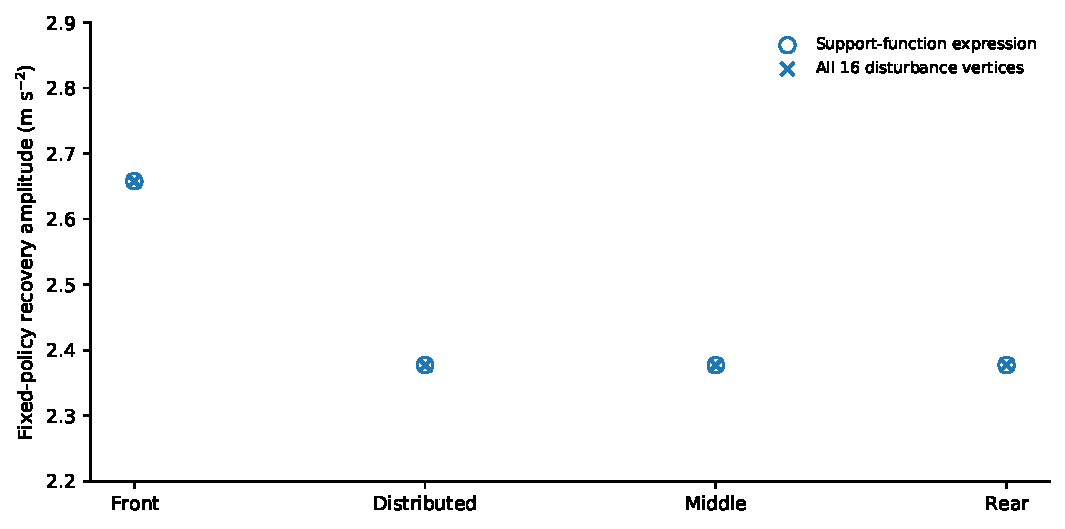
\includegraphics[width=.92\linewidth]{figS1_vertex_check.pdf}
\caption{\textbf{Support expression and disturbance vertices.} The four-coordinate disturbance box has 16 vertices. The support-function calculation and exhaustive vertex evaluation give coincident fixed-policy radii for the sampled-linear model in section S6.}
\label{fig:vertices}
\end{figure}
\begin{figure}[H]\centering
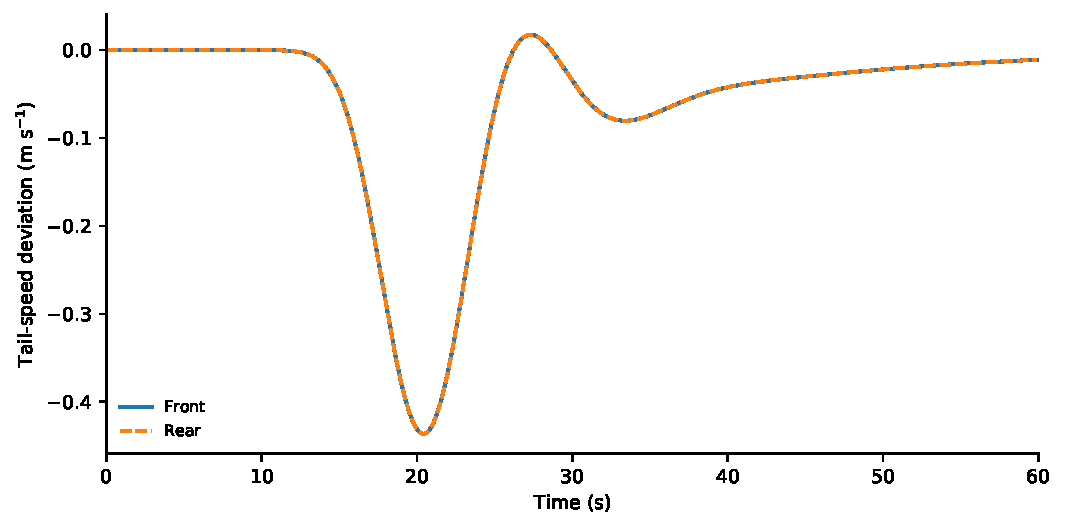
\includegraphics[width=.92\linewidth]{figS2_endpoint_response.pdf}
\caption{\textbf{Identical endpoint responses can coexist with different local limits.} At $\alpha=1\,\mathrm{m\,s^{-2}}$ and coordinate vector $(-1,-1,-1,-1)$, front and rear layouts yield overlapping tail-speed responses. The global coefficient comparison includes all four unit coordinates and all four layouts.}
\label{fig:tail}
\end{figure}

Table~\ref{tab:traceability} maps each analytical statement to its assumptions and displayed evidence.
\begin{table}[H]
\centering
\caption{Relation between analytical statements and numerical evidence. Sampled-linear reserve values concern the fixed instance of section S6. Theorem S3 applies to the stated nonlinear directed dynamics; its trajectory witnesses are distinct from the sampled-linear radii.}
\label{tab:traceability}
\small
\begin{tabularx}{\linewidth}{>{\raggedright\arraybackslash}p{.23\linewidth}>{\raggedright\arraybackslash}p{.27\linewidth}>{\raggedright\arraybackslash}X}
\toprule
Statement or formula & Assumptions and computed object & Displayed evidence\\
\midrule
Theorem~\ref{thm:reserve}, Eqs.~\eqref{eq:radius} and \eqref{eq:fullradius} & Fixed affine policy, fixed model, box disturbance; 66,072 sampled constraint rows and the separate positive-part loss term & Main Fig.~4 and Fig.~\ref{fig:vertices}\\
Theorem~\ref{thm:upper} & Relaxed admissible command set and one necessary affine row; the theorem allows nonzero control-response vector $p_r$, but the numerical obstruction uses the exact $p_r=0$ prefix case & Support-function upper-bound equation and Main Fig.~4\\
Theorem~\ref{thm:prefix} & Directed predecessor following, fixed leader trajectory and no upstream control edge & Matching first-follower obstruction for distributed, middle and rear layouts in Main Fig.~4; nonlinear prefix witnesses in Main Fig.~3\\
Proposition~\ref{prop:design} and Eq.~\eqref{eq:marginprogram} & Fixed model, active set and implementable full-horizon affine policy & Theoretical construction only; not used by the nonlinear candidate-command controllers\\
Cascade product $\prod_iG_i$ & Scalar predecessor-following factors and zero initial deviations & Fig.~\ref{fig:tail}; maximum coefficient difference $2.8\times10^{-16}$\\
Nonlinear empirical boundary & Sampled heterogeneous dynamics, requested pulse, saturation, finite grid and controller-specific closed loop & Main Figs.~2, 3 and 5; Fig.~\ref{fig:scope}\\
OVM/FVD prefix check & Same nonlinear implementation, middle/rear layouts, six paired seeds at two amplitudes; 24-run extension to the primary study & Main text and Table~\ref{tab:ovm}\\
\bottomrule
\end{tabularx}
\end{table}

\section{Nonlinear experiments}\label{sec:nonlinear}
\subsection*{Human-driving dynamics, heterogeneity and equilibrium calibration}
The nonlinear implementation uses $N$ for the number of followers and one additional external leader. The primary case has $N=40$, four active followers $\{1,14,27,40\}$, time step $\Delta t=0.1$ s and horizon 60 s. All vehicles start at $\bar v=20\,\mathrm{m\,s^{-1}}$ and 24 m net gap. For a delayed local state $(s_i,v_i,v_{i-1})$, the intelligent driver model (IDM) request is
\begin{align}
s_i^*&=s_i^0+v_iT_i+\frac{v_i(v_i-v_{i-1})}{2\sqrt{A_iB_i}},\\
f_i^{\rm IDM}&=A_i\left[1-\left(\frac{v_i}{v_i^0}\right)^4-
\left(\frac{s_i^*}{\max(s_i,0.1\ \mathrm m)}\right)^2\right].
\end{align}
The means of $(A_i,B_i,s_i^0,T_i)$ are $(1.25\,\mathrm{m\,s^{-2}},2.0\,\mathrm{m\,s^{-2}},2.0\,\mathrm m,0.9\,\mathrm s)$. Each parameter is multiplied by $1+0.12\zeta$, $\zeta\sim\mathcal U[-1,1]$, with numerical floors $(0.4,0.8,0.8,0.45)$ in the same units. The headway is then capped at $(0.95\bar s-s_i^0)/\bar v$. Defining $d_i=s_i^0+\bar vT_i$, equilibrium calibration sets
\begin{equation}
v_i^0=\bar v\left[1-(d_i/\bar s)^2\right]^{-1/4},
\end{equation}
with the bracket floored at $10^{-5}$ in code.

The alternative optimal-velocity/full-velocity-difference (OVM/FVD) request is
\begin{align}
V_i(s)&=v_i^0\frac{\tanh[(s-c_i)/w_i]+\tanh(c_i/w_i)}{1+\tanh(c_i/w_i)},\\
f_i^{\rm OVM}&=k_i^{\rm ov}\{V_i(s_i)-v_i\}+k_i^{\Delta v}(v_{i-1}-v_i).
\end{align}
The means of $(w_i,c_i,k_i^{\rm ov},k_i^{\Delta v})$ are $(6\,\mathrm m,18\,\mathrm m,0.09\,\mathrm{s^{-1}},0.55\,\mathrm{s^{-1}})$, with the same multiplicative draw and respective floors $(2\,\mathrm m,8\,\mathrm m,0.04\,\mathrm{s^{-1}},0.20\,\mathrm{s^{-1}})$. Here $v_i^0$ is recalibrated as $\bar v[1+\tanh(c_i/w_i)]/[\tanh((\bar s-c_i)/w_i)+\tanh(c_i/w_i)]$, with denominator floor $10^{-4}$. Thus neither model is forced to be string stable, but every sampled vehicle shares the declared equilibrium. The pseudorandom generator is reinitialized from the same seed in each controller run, so matched configurations regenerate the same parameter sequence.

\subsection*{Delay indexing, integration and disturbance injection}
For a continuous delay $d$, the implementation reads sample $\max\{0,k-\lceil d/\Delta t\rceil\}$. HDVs evaluate their car-following rule at a state delayed by 0.7 s. CAV measurements are delayed by 0.2 s; after saturation the command is delayed by a further 0.2 s in the primary case; and realised CAV acceleration follows a first-order lag of 0.35 s. The sensitivity cases change only command delay to 0 or 0.4 s.

Each step first forms and constrains the leader request. All followers then read positions, speeds and accelerations from the same frozen current or delayed time index. HDV or controlled requests are formed from that snapshot, with an internal disturbance added when applicable; no newly updated follower state is used by another follower in the same step. Requests are clipped to $[-5,2.5]\,\mathrm{m\,s^{-2}}$, delayed CAV commands are retrieved, and actuator lag, jerk clipping and acceleration clipping are applied. Speeds are updated using the new acceleration and positions using the new speed; gaps and first-occurrence logs follow. CAV lag uses $(u^{\rm delayed}-a_i)/\max(0.35,\Delta t)$, whereas an HDV uses $(u^{\rm sat}-a_i)/\Delta t$. Realised acceleration is limited to $[-4.5,2.0]\,\mathrm{m\,s^{-2}}$, speed is projected to $[0,35]\,\mathrm{m\,s^{-1}}$, and jerk magnitude is limited to $5\,\mathrm{m\,s^{-3}}$. A nonpositive gap sets a collision flag, but integration continues to preserve a failure record; post-collision states have no physical interpretation.

The leader request begins at 5 s and is $-\alpha$ for 1.5 s followed by $+\alpha$ for 1.5 s. It is clipped to the acceleration limits and reaches them through the same $5\,\mathrm{m\,s^{-3}}$ jerk limit. After the 3 s pulse, the leader requests $0.8(\bar v-v_0)$. Thus $\alpha$ is a requested acceleration amplitude; for $\alpha>2\,\mathrm{m\,s^{-2}}$ the positive leg saturates. In the internal-source test, the requested waveform is added to follower 8's ordinary delayed HDV request before saturation. Follower 8 is not active in the even set $\{1,14,27,40\}$. This protocol differs from the homogeneous box disturbance used for the exact linear result in section S6. At requested $\alpha=2.1\,\mathrm{m\,s^{-2}}$, the six source-response trajectories give leader speed drop and negative-acceleration integral of 3.15 $\mathrm{m\,s^{-1}}$ over 1.9 s. Follower 8 gives speed drops 2.699--2.765 $\mathrm{m\,s^{-1}}$ and negative-acceleration integrals 3.163--3.222 $\mathrm{m\,s^{-1}}$ over 50.1--51.1 s. The long latter duration includes small closed-loop deceleration after the injected pulse and is not a pulse-duration match.

\subsection*{Implemented nonlinear controllers}
For all active vehicles, the adaptive-cruise-control (ACC) request is
\begin{equation}
u_i^{\rm ACC}=0.18\{s_i-(3+1.05v_i)\}+0.75(v_{i-1}-v_i),
\end{equation}
and the implemented wave-damping baseline adds $(0.35\,\mathrm{s^{-1}})(20\,\mathrm{m\,s^{-1}}-v_i)$. In the ACC expression, the gap gain is $0.18\,\mathrm{s^{-2}}$, the relative-speed gain is $0.75\,\mathrm{s^{-1}}$, and the target gap is $3\,\mathrm m+(1.05\,\mathrm s)v_i$. This comparator is named by its implemented function and is not asserted to reproduce a specific published field controller.

The endpoint-screened and margin-priority endpoint-screened controllers share 31 commands $u_j=-5+0.25j$, $j=0,\ldots,30$, and an endpoint horizon $H=1.2$ s. With $\rho=1-\exp[-H/\max(0.35,\Delta t)]$ they evaluate
\begin{equation}
a_j^+=\operatorname{clip}\{a_i+\rho(u_j-a_i),-4.5,2\},\quad
v_j^+=v_i+Ha_j^+,
\end{equation}
\begin{equation}
s_j^+=s_i+H(v_{i-1}-v_i)+\tfrac12H^2(a_{i-1}-a_j^+).
\end{equation}
Here $\operatorname{clip}(x,l,u)=\min\{u,\max\{l,x\}\}$. The input state has already undergone information delay. The predictor holds predecessor acceleration constant and uses an endpoint acceleration produced by a first-order-lag formula, but it does not integrate that lag over the horizon or propagate the separate command-delay register or jerk clipping. The feasible pool satisfies $s_j^+\geq5$ m and $0\leq v_j^+\leq35\,\mathrm{m\,s^{-1}}$; if this pool is empty, all candidates are retained. The common dimensionless tracking cost is
\begin{equation}
C_j=\left\{\frac{s_j^+-24\,\mathrm m}{8\,\mathrm m}\right\}^2+
\left\{\frac{v_j^+-20\,\mathrm{m\,s^{-1}}}{4\,\mathrm{m\,s^{-1}}}\right\}^2+
0.025\left\{\frac{u_j}{1\,\mathrm{m\,s^{-2}}}\right\}^2.
\end{equation}
Endpoint-screened control selects the first minimum in ascending command order. Margin priority retains candidates with $C_j\leq\min C+0.01$ and maximizes the smallest of
\begin{equation}
\frac{s_j^+-4}{20},\ \frac{v_j^+}{20},\ \frac{35-v_j^+}{15},\
\frac{2-a_j^+}{2},\ \frac{a_j^++4.5}{4.5},\
\frac{2.5-u_j}{2.5},\ \frac{u_j+5}{5}.
\end{equation}
Remaining ties are resolved by smaller tracking cost and then ascending command order. The first minimum $C_{\min}$ is taken over the feasible pool, or over all 31 candidates after the empty-pool fallback. The 5-m quantity controls pool admission, whereas the displayed secondary gap margin is measured from the specified 4-m safety minimum. The tolerance 0.01 was selected on development seed 3. This online controller is distinct from the full-horizon affine program in section S5.

For Fig.~\ref{fig:constraintuse}, realised state utilisation is the maximum of $(24-s_i)/20$, $(20-v_i)/20$ and $(v_i-20)/15$. Actuator utilisation is the maximum of $a_i/2$, $-a_i/4.5$, $|\Delta a_i/\Delta t|/5$, $u_i^{\rm sat}/2.5$ and $-u_i^{\rm sat}/5$. Values are reported for followers only. An individual signed component can be negative when moving away from its boundary. Because complementary speed and acceleration components are included, the displayed maximum is nonnegative. Recovery events are computed separately.

The primary amplitude grid is
\[
\{0,0.25,1.0,1.5,1.7,1.8,1.9,2.0,2.1,2.5,3.0,3.5,4.0,4.5\}\,\mathrm{m\,s^{-2}}.
\]
All five controllers use 12 paired seeds in the core range; high-amplitude extension is available only for the two endpoint-screened methods that remained successful at 2.5. Front, middle and rear layout comparisons use 12 seeds through $2.5\,\mathrm{m\,s^{-2}}$ and 6 seeds at larger amplitudes. The even primary layout uses 12 seeds throughout. Other source, model, delay and follower-count extensions use 6 seeds per evaluated cell. No rate rebound was observed in the reported aggregate grids. The evaluated amplitudes and paired subsets are retained in the run records.

The six seeds present in every high-amplitude placement cell are 97, 113, 131, 149, 167 and 191. Restricting the lower-amplitude cells to this common subset leaves the descriptive placement endpoints unchanged: front reaches the ceiling, middle has 3/6 recoveries at 1.5 and 0/6 at 1.7, and rear has 1/6 at 1.5 and 6/6 at 1.0. This restricted-seed comparison holds seed composition fixed.

Table~\ref{tab:nonlinear} lists the principal empirical boundaries and their direct interpretation.
\begin{table}[H]\centering
\caption{Principal nonlinear results. The $\geq4.5$ entries denote aggregate 50\% grid estimates that reach the tested amplitude ceiling.}
\label{tab:nonlinear}
\begin{tabularx}{\linewidth}{>{\raggedright\arraybackslash}p{.29\linewidth}>{\centering\arraybackslash}p{.22\linewidth}>{\raggedright\arraybackslash}X}\toprule
Case and method & Boundary ($\mathrm{m\,s^{-2}}$) & Direct interpretation\\\midrule
Primary: human / ACC & $1.0/1.0$ & Both fail in at least 11/12 seeds at $\alpha=1.5$.\\
Primary: implemented wave damping & $1.7$ & Recovery rate is 7/12 at 1.7 and 4/12 at 1.8.\\
Primary: endpoint-screened / margin-priority & $\geq4.5/\geq4.5$ & Each recovers 11/12 at the ceiling.\\
Margin layout: front / even / middle / rear & $\geq4.5/\geq4.5/1.5/1.0$ & Both reach the scan ceiling and share earliest active follower 1.\\
Margin source: leader / follower 8 & $\geq4.5/2.1$ & Moving the source changes the recorded boundary.\\
Margin human model: IDM / OVM--FVD & $\geq4.5/1.0$ & The recorded boundary is lower for OVM/FVD.\\
Margin command delay: 0 / 0.2 / 0.4 s & $\geq4.5/\geq4.5/4.0$ & Other delay channels are unchanged.\\\bottomrule
\end{tabularx}
\end{table}

At $\alpha=4.5$, the endpoint-screened and margin-priority controllers both recover 11/12 seeds. Paired trajectories provide differences for all 12 seeds. Margin-priority minus endpoint-screened endpoint gap error has median $-1.096$ m and a 10,000-resample seed-bootstrap 95\% interval for the median of $[-1.483,-0.714]$ m. The final-3-s maximum gap-error difference has median $-0.718$ m and interval $[-0.990,-0.436]$ m. Normalized distance-deficit difference has median 0.00218 and interval [0.00207, 0.00240]. Every one of the 12 pairs has the same direction for all three outcomes. These descriptive intervals preserve seed pairing.

\subsection*{Boundary records, regression features and failure accounting}
For each seed and configuration, the recorded response is the largest successful evaluated amplitude, not a connected-prefix estimator. A separate flag tests whether any success follows a failure in the ordered grid; none of the 156 per-seed boundary records is flagged. Aggregate 50\% endpoints are the largest amplitudes with recovery in at least half of the available seeds. Successful observations at the largest evaluated amplitude are right-censored, but the regressions treat their recorded endpoint as a numeric label rather than using a censoring-aware model.

The prediction analysis keeps whole configurations in one split. The 36 development records use even/front leader cases, the follower-8 source and zero command delay. The 36 test records use middle/rear layouts, 0.4 s command delay and OVM/FVD dynamics. The 36 records within either split arise from a small set of configurations and are not independent configuration draws. For each record, zero-amplitude and $0.25\,\mathrm{m\,s^{-2}}$ runs define $m_0$, the predicted bottleneck margin at zero pulse, and $m_{0.25}$ at the probe. The finite-difference slope is $q=(m_{0.25}-m_0)/(0.25\,\mathrm{m\,s^{-2}})$. The directional reserve proxy is $-m_0/q$ for $q<-10^{-9}$ in the specified units and otherwise the largest core-grid amplitude, then clipped to $[0,5]\,\mathrm{m\,s^{-2}}$. Its ordinary least-squares design contains an intercept and the unstandardized variables reserve proxy, small-pulse internal gain, integer distance from the source to the nearest active CAV, and command delay. Each comparator uses an intercept and its named scalar feature. Predictions are clipped to $[0,5]$ before errors and exceedance fractions are calculated.

The directional feature has test mean absolute error (MAE) $3.1715\,\mathrm{m\,s^{-2}}$ and recorded-boundary exceedance fraction 0.8333. Distance to the nearest active vehicle gives 1.3023 and 0.3056; small-pulse gain gives 1.4962 and 0.9722. The exceedance fraction compares predictions with recorded grid endpoints. Coarse and ceiling-censored labels preclude interpreting it as a collision probability or certification error. No failed run exists at the $0.25\,\mathrm{m\,s^{-2}}$ probe, so a first-failure hit rate is not estimated. The 0.01 margin tolerance was chosen with development seed 3, which also belongs to the primary descriptive set; this tuning is disclosed rather than treated as independent validation.

The primary study contains 1,848 closed-loop runs. Wilson intervals use one Bernoulli recovery outcome per run; trajectory frames are not treated as independent samples. Failure criteria are multilabel: path safety, terminal speed, terminal gap, terminal acceleration and distance-budget failures can coexist. A deterministic priority is retained only for optional single-class summaries. In the representative $\alpha=4.5\,\mathrm{m\,s^{-2}}$ run, implemented wave damping first crosses the specified 4-m gap minimum at follower 7 and 17.2 s and collides at follower 8 and 19.3 s. Its terminal and total-loss values after collision derive from numerical continuation and are not interpreted as physical outcomes. Trapezoidal integration of pre-collision deficits through 19.3 s gives 0.00905, below the 0.03 total budget; the full-horizon budget result is not physically evaluable. Both endpoint-screened trajectories meet all five criteria. Their follower-only peak jerk values are 1.407 and $2.375\,\mathrm{m\,s^{-3}}$; the all-vehicle metric is $5\,\mathrm{m\,s^{-3}}$ because the requested leader pulse contacts its jerk limit. Contact with a declared actuator limit is logged but is not by itself classified as recovery failure.

\subsection*{Exact layout indices and directional classification}
Table~\ref{tab:layouts} records the indices used in the reported configurations. Online policies act only at these existing indices and cannot reorder vehicles.

\begin{table}[H]\centering
\caption{Active follower indices in the sampled-linear and nonlinear calculations. The external leader is index 0.}
\label{tab:layouts}
\small
\begin{tabularx}{\linewidth}{>{\raggedright\arraybackslash}p{.18\linewidth}>{\centering\arraybackslash}p{.13\linewidth}>{\raggedright\arraybackslash}p{.19\linewidth}>{\raggedright\arraybackslash}X}
\toprule
Model & $N$ & Layout & Active follower indices\\
\midrule
Sampled linear & 12 & Front & 1, 2\\
Sampled linear & 12 & Distributed & 3, 7\\
Sampled linear & 12 & Middle & 6, 7\\
Sampled linear & 12 & Rear & 11, 12\\
Nonlinear & 20 & Even & 1, 20\\
Nonlinear & 40 & Front & 1, 2, 3, 4\\
Nonlinear & 40 & Even & 1, 14, 27, 40\\
Nonlinear & 40 & Middle & 19, 20, 21, 22\\
Nonlinear & 40 & Rear & 37, 38, 39, 40\\
Nonlinear & 80 & Even & 1, 12, 24, 35, 46, 57, 69, 80\\
\bottomrule
\end{tabularx}
\end{table}

For active set $\mathcal C$, let $j=\min\mathcal C$ and $P=\{1,\ldots,j-1\}$. The leader is 0 and indices increase rearward, so influence in this model follows $0\rightarrow1\rightarrow\cdots\rightarrow N$. The front and even $N=40$ sets have empty $P$. The middle and rear sets have prefixes $1{:}18$ and $1{:}36$. The nonlinear code is strictly predecessor following, the leader path is external, and these prefix vehicles have no control input. Theorem~\ref{thm:prefix} therefore applies without linearization.

Each declared layout--amplitude--seed cell is assigned exactly one category: A, recovered by the evaluated controller; B, its failure with a logged first prefix crossing below the specified 4-m safety minimum; C, evaluated failure without such a prefix witness; or D, unevaluated. Over 168 declared cells per layout, front has 144 evaluated (A=144, B=C=0, D=24), even 168 (A=167, B=0, C=1, D=0), middle 144 (A=42, B=93, C=9, D=24), and rear 144 (A=37, B=105, C=2, D=24). Thus B accounts for 93/102 middle failures and 105/107 rear failures. Repeated amplitudes and common seeds are correlated, so these counts describe the evaluated grid rather than independent samples. D is a missing-evaluation label, not a physical phase; C remains unresolved by the prefix test.

Across all 198 B records, the earliest logged prefix safety or collision event is a positive-gap crossing below 4 m in the uncontrolled prefix and precedes any prefix collision. Matched configurations reconstruct the same parameter sequence from their fixed seeds. These trajectory-specific witnesses establish obstruction under the directed model and declared histories.

The discrete update is $x_{i,k+1}=x_{i,k}+\Delta t\,v_{i,k+1}$, with $0\le v_{i,k+1}\le35\,\mathrm{m\,s^{-1}}$ and $\Delta t=0.1$ s. Hence one-step net-gap decrease is at most 3.5 m. A first crossing from a positive gap to a nonpositive gap must therefore follow a prior sample below 4 m. More directly, the 198 logged first prefix crossings are already positive-gap safety violations before prefix collision. A collision of a vehicle behind $P$ does not alter this autonomous prefix subsystem in the declared model. The structural statement remains conditional on the fixed model, histories, leader path, parameters and active set, and it rules out prevention of the prefix violation under that setup rather than asserting inevitable collision.

The primary OVM/FVD grid evaluates only the even layout, for which the first CAV is follower 1 and the uncontrolled prefix is empty. A 24-run extension evaluates middle and rear layouts at two requested amplitudes with six paired seeds, the same margin-priority endpoint-screened controller and otherwise identical configuration values. Table~\ref{tab:ovm} gives the resulting descriptive categories. Here a B witness requires a positive first prefix gap below 4 m before any collision in the chain. All three OVM/FVD B records match the first below-bound sample in their prefix gap trajectories at 52.4--59.3 s; none has a collision. The four matched IDM B records also precede the first chain collision. The remaining failures are C and remain unresolved by this obstruction test.

\begin{table}[H]\centering
\caption{Cross-model prefix classification. Each row has six paired seeds at the requested amplitude. A is observed recovery; B is a pre-collision prefix-safety witness; C is an observed failure unresolved by this test. Repeated seeds across amplitudes are correlated and these counts are not population estimates. IDM cells belong to the primary study; OVM/FVD cells belong to the 24-run extension.}
\label{tab:ovm}
\begin{tabular}{llcc}\toprule
Layout & Requested $\alpha$ ($\mathrm{m\,s^{-2}}$) & IDM A/B/C & OVM/FVD A/B/C\\\midrule
Middle & 1.0 & 6/0/0 & 6/0/0\\
Middle & 1.5 & 3/0/3 & 3/0/3\\
Rear & 1.0 & 6/0/0 & 0/0/6\\
Rear & 1.5 & 1/4/1 & 0/3/3\\\bottomrule
\end{tabular}
\end{table}

\subsection*{Source, chain-length and driver-model scope}
Three comparisons delimit transfer of the reported boundaries (Fig.~\ref{fig:scope}). At requested $\alpha=2.1\,\mathrm{m\,s^{-2}}$, the realized leader speed drop is 3.15 $\mathrm{m\,s^{-1}}$, whereas follower 8 drops by 2.699--2.765 $\mathrm{m\,s^{-1}}$ across six paired realizations. The internal pulse is added to a delayed car-following request before saturation, so equal requested amplitudes do not produce identical source responses. At requested $\alpha=4.0\,\mathrm{m\,s^{-2}}$, seed 97, the number of followers reaching at least $1\,\mathrm{m\,s^{-1}}$ speed deviation before 60 s is 19/20, 17/40 and 16/80. Full-chain normalization of distance deficit can therefore dilute a disturbance that has not reached most of a long chain by the deadline. Active control count and parameter draws also change with $N$ in these configurations. Finally, IDM and OVM/FVD share the calibrated equilibrium and have similar but nonidentical mean local derivatives; this comparison does not separate linear-response differences from higher-order nonlinear effects.

\subsection*{Endpoint approximation and collision handling}
For the 12 paired seeds at requested $\alpha=4.5\,\mathrm{m\,s^{-2}}$, 24 endpoint-screened trajectory evaluations provide 601 time points each. A 12-step prediction horizon leaves 589 eligible decision indices; four active vehicles yield $24\times589\times4=56{,}544$ selected-command comparisons. The final 12 indices lack a complete prediction window and are excluded. No eligible decision has an empty candidate pool. No selected candidate passing the 5-m/speed screen fails the corresponding discrete counterfactual endpoint check.

The screening-model speed increment is $Ha^+$. For comparison, an exact constant-command, unclipped first-order lag gives
\begin{equation}
\Delta v_{\rm lag}=uH+(a-u)\tau_a(1-\exp[-H/\tau_a]).
\end{equation}
For $a=0$, $u=1\,\mathrm{m\,s^{-2}}$, $H=1.2$ s and $\tau_a=0.35$ s, the screening-model increment is 1.1611 $\mathrm{m\,s^{-1}}$ and the exact lag integral is 0.8614 $\mathrm{m\,s^{-1}}$. The discrete comparison holds the selected command over 12 ego updates after already queued commands, applies clipping and speed projection, and uses the predecessor's recorded future position. It is a conditional counterfactual under that predecessor path, not the ego's later closed-loop state. Across all eligible decisions, the 95th percentiles of absolute screening-versus-discrete differences are 0.0762 $\mathrm{m\,s^{-1}}$ for speed and 0.208 m for gap. Restricting to nontrivial commands or the 5--15 s pulse window gives 13,741 decisions, mean absolute gap difference 0.1478 m and maximum 2.8191 m (Fig.~\ref{fig:endpoint}).

No speed projection occurs in the 24 paired endpoint-screened trajectories, including failed seed 11. In the representative wave-damping trajectory, 2,543 projection events occur only after its first collision; none occurs before the first 4-m safety crossing or collision. The displayed physical trajectory is truncated at collision, whereas numerical continuation retains the failure record.

\begin{figure}[H]\centering
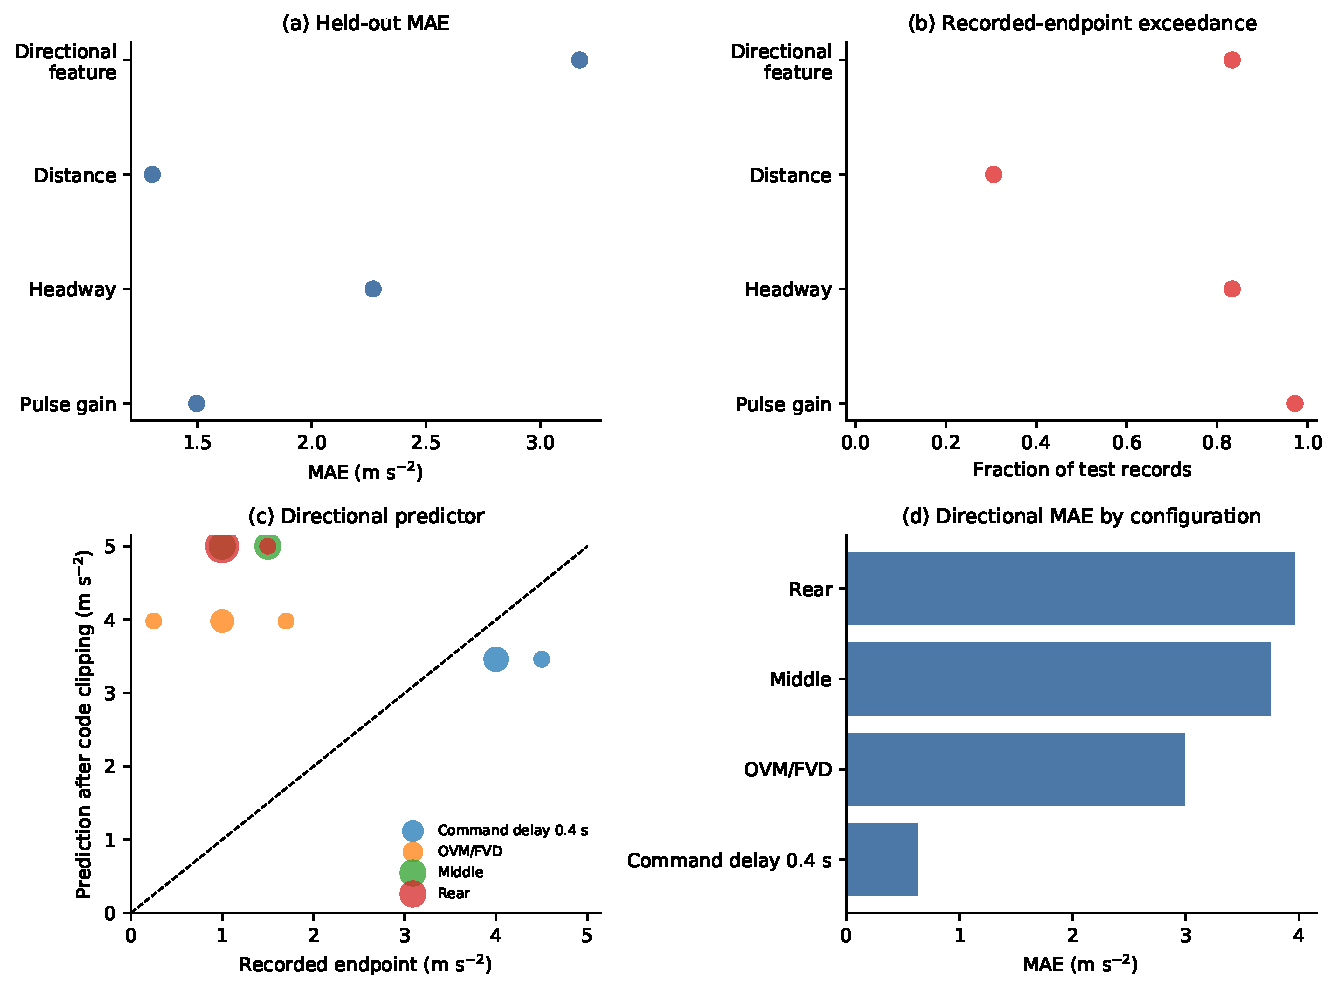
\includegraphics[width=.95\linewidth]{figS3_predictor_diagnostics.pdf}
\caption{\textbf{Held-configuration boundary-prediction diagnostics.} Repeated points retain their multiplicity; ceiling-limited recorded endpoints are treated as numeric regression labels, not by a censoring-aware method. The directional model's development design has rank 5/5 but unstandardized condition number 64,447; its reserve proxy is clipped at the upper limit in 30/36 development records.}
\label{fig:predictor}
\end{figure}

\begin{figure}[H]\centering
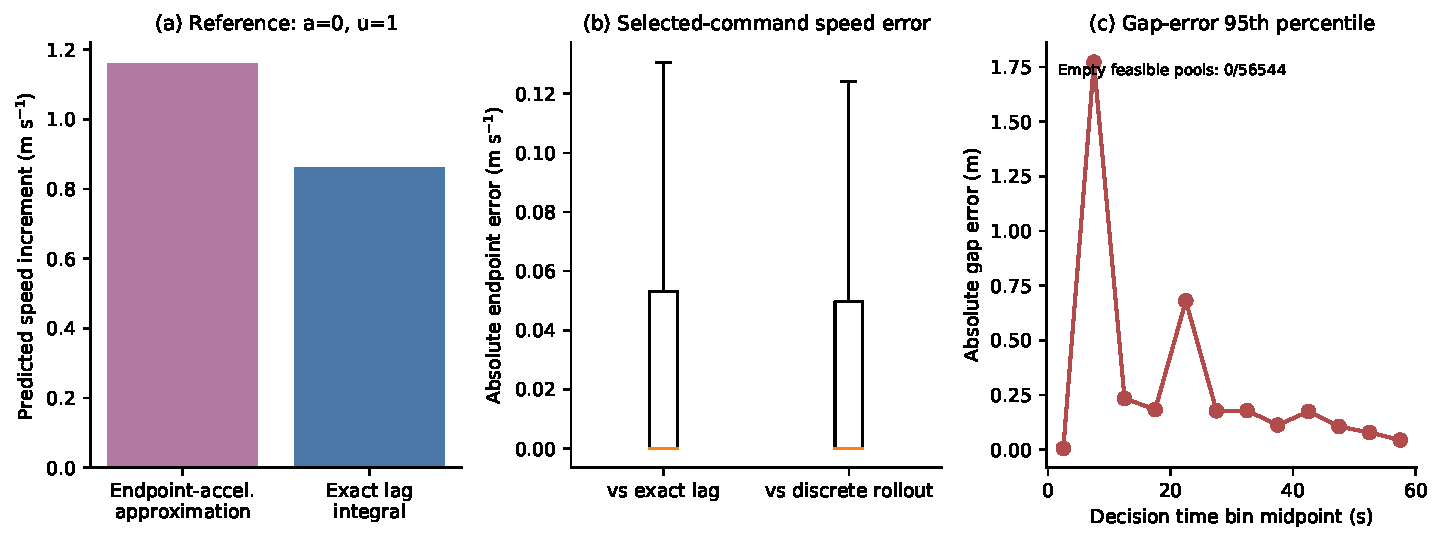
\includegraphics[width=.95\linewidth]{figS4_endpoint_approximation.pdf}
\caption{\textbf{Endpoint-approximation validation.} Differences between the screening endpoint-acceleration model and exact constant-command lag or a discrete held-command counterfactual are evaluated at 56,544 selected decisions from 24 paired trajectories. Panel (b) shows the 13,741-decision nontrivial-command/pulse subset: boxes mark quartiles, whiskers extend to 1.5 interquartile ranges and fliers are hidden for legibility; the full maximum gap discrepancy is reported in the text. Panel (c) gives the 95th percentile of absolute gap error within each 5-s decision-time bin. Empty-pool and screen-disagreement counts are zero in the eligible subset.}
\label{fig:endpoint}
\end{figure}

\begin{figure}[H]\centering
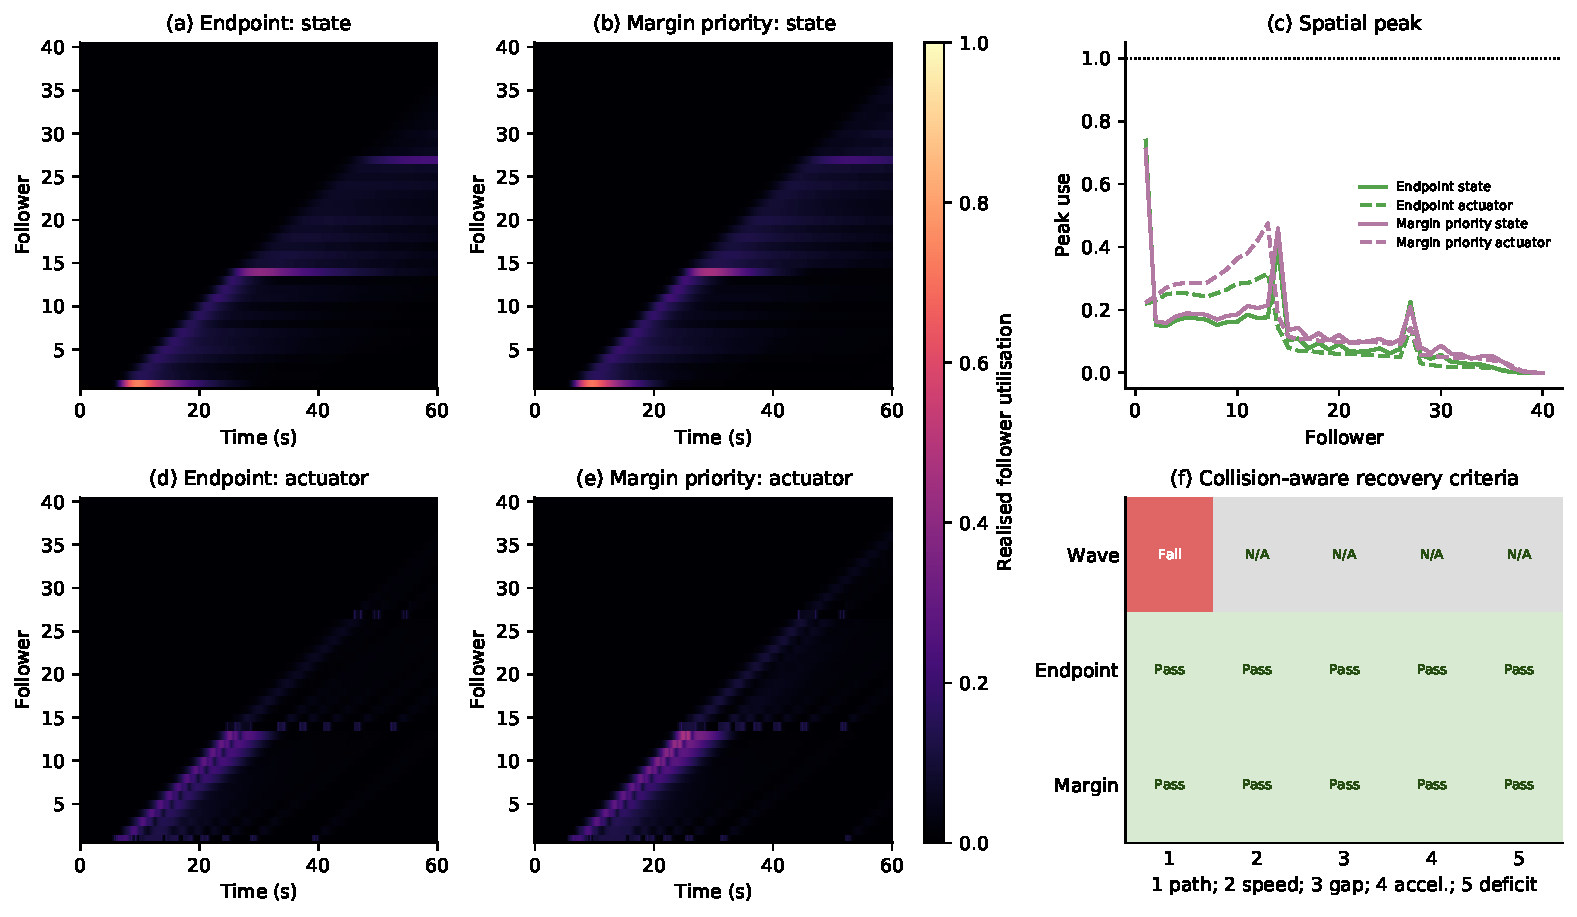
\includegraphics[width=.95\linewidth]{figS5_constraint_use.pdf}
\caption{\textbf{Constraint use and recovery criteria in representative trajectories.} State and actuator utilization are separated by follower. Individual signed components can be negative, but their displayed maximum is nonnegative. In panel (f), wave-damping path safety fails before collision; terminal speed, gap, acceleration and full-horizon distance deficit are marked N/A because numerical continuation after collision has no physical terminal interpretation. Pre-collision normalized deficit is 0.00905, below the 0.03 budget at that time. The two collision-free controllers pass all five criteria.}
\label{fig:constraintuse}
\end{figure}

\begin{figure}[H]\centering
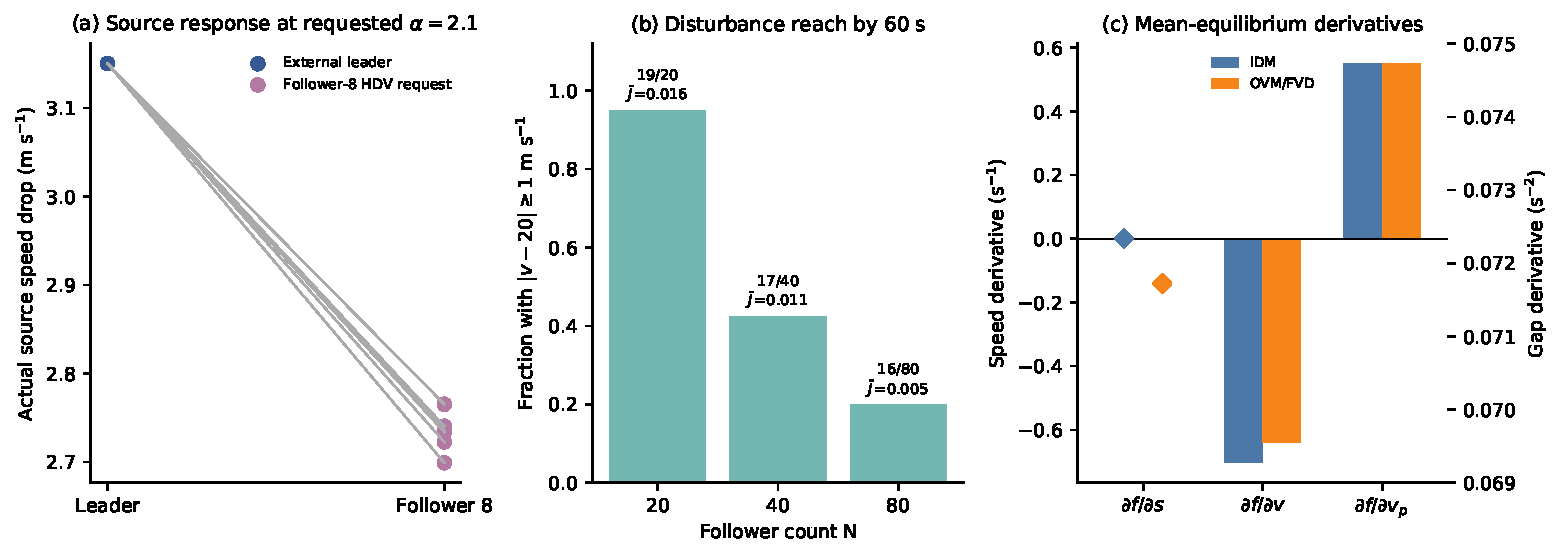
\includegraphics[width=.95\linewidth]{fig5_scope_diagnostics.pdf}
\caption{\textbf{Scope of source, chain-length and driver-model comparisons.} (a) Realized source-speed drops for an external leader and additive follower-8 HDV request at the same requested amplitude. (b) Followers reaching the $1\,\mathrm{m\,s^{-1}}$ deviation threshold by 60 s at requested $\alpha=4.0\,\mathrm{m\,s^{-2}}$, seed 97, under margin-priority control; counts and full-$N$ normalized deficit are shown. (c) Mean-equilibrium derivatives of IDM and OVM/FVD; speed derivatives use the left axis ($\mathrm{s^{-1}}$) and gap-derivative diamonds the right axis ($\mathrm{s^{-2}}$).}
\label{fig:scope}
\end{figure}

\end{document}
